\documentclass[a4paper,12pt]{report}
\usepackage[utf8]{inputenc}
\usepackage[francais]{babel}
\usepackage{fancyhdr}
\usepackage{graphicx}
\usepackage{tikz}
\usetikzlibrary{calc}
\usepackage{listings}
\usepackage{xcolor}
\definecolor{grey}{rgb}{0.9,0.9,0.9}
\usepackage{titlesec}
\usepackage{verbatim}
\usepackage{listings}
\usepackage{textcomp}
\usepackage{hyperref}
\usepackage{longtable}
\usepackage{colortbl}
\usepackage{amssymb}


\frenchbsetup{StandardLists=true}
\newcommand{\marge}{18mm}
\usepackage[left=\marge,right=\marge,top=\marge,bottom=\marge]{geometry}
\pagestyle{fancy}
\setlength{\headheight}{14pt}
\chead{
  \textbf{Monôme:} Douaille Erwan 
    \hspace{2em}
  \textbf{Groupe:} M2 Info IVI}
\renewcommand{\headrulewidth}{1pt}
\linespread{1}
\setlength{\columnseprule}{0.2pt}
\definecolor{javakeyword}{rgb}{0,0,0.5}
\definecolor{javastring}{rgb}{0,0.5,0}
\definecolor{javacomment}{rgb}{0.5,0.5,0.5}
\lstdefinestyle{C++}{
   language=C++, basicstyle=\footnotesize,       % the size of the fonts that are used for the code
  numbers=left,                   % where to put the line-numbers
  numberstyle=\tiny\color{gray},  % the style that is used for the line-numbers
  stepnumber=1,                   % the step between two line-numbers. If it's 1, each line
                                  % will be numbered
  numbersep=5pt,                  % how far the line-numbers are from the code
  backgroundcolor=\color{white},  % choose the background color. You must add \usepackage{color}
  showspaces=false,               % show spaces adding particular underscores
  showstringspaces=false,         % underline spaces within strings
  showtabs=false,                 % show tabs within strings adding particular underscores
  frame=single,                   % adds a frame around the code
  rulecolor=\color{black},        % if not set, the frame-color may be changed on line-breaks within not-black text (e.g. commens (green here))
  tabsize=2,                      % sets default tabsize to 2 spaces
  captionpos=b,                   % sets the caption-position to bottom
  breaklines=true,                % sets automatic line breaking
  breakatwhitespace=false,        % sets if automatic breaks should only happen at whitespace
  title=\lstname,                 % show the filename of files included with \lstinputlisting;
   stringstyle=\color{javastring},
   keywordstyle=\color{javakeyword}\ttfamily\textbf,
   commentstyle=\color{javacomment}\ttfamily\textit
 }
\begin{document}



\makeatletter
\begin{titlepage}
\centering
\vspace{-10em}
{\LARGE \textbf{\textsc{Rapport de Projet RVI}}}\\
\vspace{3em}

\includegraphics[scale=0.6]{image/thalassa.png}\\
\vspace{3em}
{\LARGE \textsc{Projet Thalassa: simulation de plongée sous-marine}}\\

\vspace{8em}
Par\\
\vspace{1em}
{\LARGE \@author}\\

\vspace{2em}



\begin{tikzpicture}[remember picture,overlay]

\node [below left,xshift=-1cm, yshift=4cm] at (current page.south east){
\includegraphics[scale=0.6]{image/ustl1.png}};

\end{tikzpicture}
\end{titlepage}
\makeatother

\sloppy

\setcounter{page}{1} 
\newpage

\section*{Introduction}

Lors de la séance précédente, nous avons observé comment obtenir les points d'une image dans un autre repére (autre image de la stéréo). Dans les images actuelles nous sommes dans une \textit{configuration canonique}. Cela veut dire que un point dans l'image de droite se trouve sur la même droite épipolaire que le point correspondant de l'image de gauche. Avec cette simplification nous pouvons nous permettre de faire de la correspondance pour l'ensemble des pixels des deux images.


\begin{figure}[!ht]
	\center
	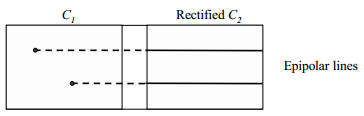
\includegraphics[scale=0.5]{./image/epipolar2.png}
	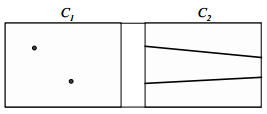
\includegraphics[scale=0.5]{./image/epipolar1.png}
	\caption{\textit{Gauche}, configuration canonique, \textit{droite}, configuration quelconque}
\end{figure}


 Pour calculer les similarités ils nous faut simplement appliquer un décalage, pour pouvoir obtenir la même partie visible de l'image de droite dans l'image de gauche; dans le cas où l'image de gauche est l'image de référence.

Pour déterminer la similarité des images nous allons donc utiliser la méthode de calcul SSD et nous vérifierons les calculs en déterminant les disparités des images.

\section*{Similarité par SSD}

Dans cette partie nous avons pour but de déterminer la similarité des images droite et gauche

Dans \textit{iviLeftDisparityMap} nous avons deux structures de données, \textit{mSSD} et \textit{mMinSSD}. Ces deux matrices vont contenir des informations relatives à l'image de gauche et de droite.

\begin{itemize}
	\item \textbf{mMinSSD} contient les valeurs minimales de décalages sur un pixel donné
	\item \textbf{mSSD} contient les valeurs de décalages (somme des différences au carré d'un pixel de droite décalé pour l'image de gauche) dans une zone autour du pixel courrant, \textit{voir formule ci-dessous}
\end{itemize}

Pour calculer \textit{mSSD} il nous faut compléter la fonction \textit{iviComputeLeftSSDCost}, qui va parcourir les deux images et calculer la somme des différences.

\begin{figure}[!ht]
	\center
	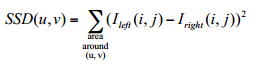
\includegraphics[scale=0.8]{./image/ssdEqua.png}
\end{figure}


Voici comment nous avons procédé:
\begin{lstlisting}[style=C++]
Mat iviComputeLeftSSDCost(const Mat& mLeftGray, const Mat& mRightGray, int iShift, int iWindowHalfSize) {
    Mat mLeftSSDCost(mLeftGray.size(), CV_64F);
    double * ptr;
     for (int x = iWindowHalfSize ; x < mLeftGray.size().height-iWindowHalfSize; x++){
        ptr = mLeftSSDCost.ptr<double>(x);
        for (int y = iWindowHalfSize; y < mLeftGray.size().width-iWindowHalfSize; y++) {
            for (int i = -iWindowHalfSize; i <= iWindowHalfSize; i++)
                for (int j = -iWindowHalfSize; j <= iWindowHalfSize; j++)
                    *ptr += pow(mLeftGray.row(x+i).at<uchar>(y+j)- mRightGray.row(x+i).at<uchar>(y+j-iShift), 2.);
        ptr++;
        }
     }
     return mLeftSSDCost;
}
\end{lstlisting}

Nous parcourons l'image de référence (içi gauche) et nous parcourons la zone autour de notre pixel (\textit{cf iWindowHalfSize}). Lors de ce parcours nous ajoutons à notre pointeur la somme des différences calculées. Le décalage (\textit{iShift}) est nécessaire pour "plaquer" l'image de droite sur notre image de référence pour faire correspondre les pixels de l'image. 

Une fois cette partie obtenue nous comparons ces valeurs aux valeurs contenue dans \textit{mMinSSD}. Dans le cas ou ces valeurs sont plus petites que celles contenues dans \textit{mMinSSD} nous affectons les valeurs de \textit{mMinSSD} à \textit{mSSD}. Cette opération nous permet d'avoir les coûts en décalage minimum.

Dans la partie suivante nous aurons besoin de deux images pour pouvoir les comparer. Pour obtenir cette seconde image, nous aplpiquons le même traitement que \textit{iviLeftDisparityMap} mais en prenant pour image de référence l'image de droite. Ce traitement sera effectué dans \textit{iviRightDisparityMap}.

Voici un aperçu de ce que nous obtenons avec ces deux méthodes:

\begin{figure}[!ht]
	\center
	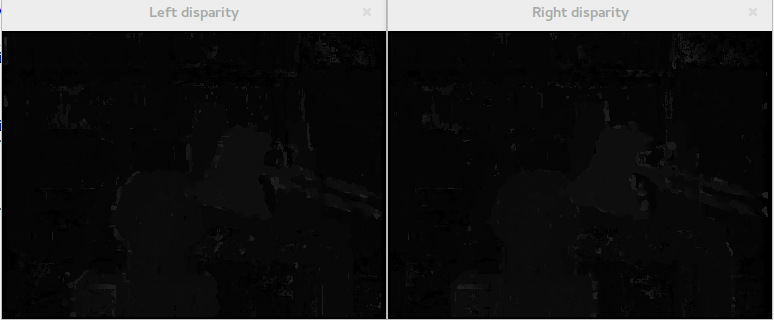
\includegraphics[scale=0.6]{./image/disparity.png}
\end{figure}

Nous pouvons observer que l'on obtient bien les formes de la lampe et le visage, principalement. Pourquoi ces deux objets ressortent plus que les éléments d'arrière plan ?

Ce "problème" est dûe de la proximité de ces deux derniers éléments.

\begin{figure}[!ht]
	\center
	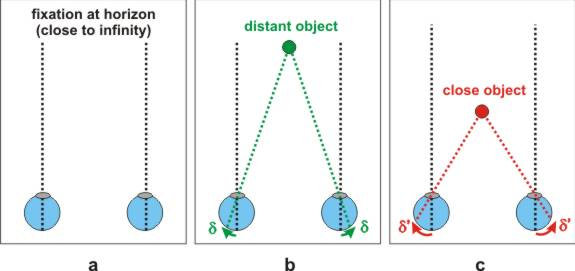
\includegraphics[scale=2]{./image/stereo.jpg}
	\caption{Vision stéréo}
\end{figure}

L'image ci-dessus illustre parfaitement ce problème. Plus les objets sont proches des 2 caméras, plus l'angle de vision va changer, ce qui aura pour effet d'avoir une vue différente des 2 objets et aura pour effet, grâce au calcul de similarité, de les démarquer.

\section*{Vérification gauche-droite}

Comme dit précédemment, \textit{iviRightDisparityMap} et \textit{iviRightSSDCost} ont dûe être créées. Elles sont proches des fonctions liées à la partie Left.

Dans cette partie notre objectif est de déterminer une carte des disparités entre l'image de gauche et l'image de droite.

L'image ci-dessous est ce que nous obtenons pour le calcul de la disparité. 
\begin{figure}[!ht]
	\center
	\includegraphics[scale=0.6]{./image/disparity2.png}
\end{figure}

Si l'image est correctement calculée, on sauvegarde la valeur de l'image des disparité gauche dans la nouvelle structure, autrement rien n'est sauvegardé. Ça nous permet d'obtenir une image de référence filtrée par l'image de droite (dans notre cas).

Pour savoir si une image est correctement calculée, nous avons utilisé la formule du cours:

\begin{figure}[!ht]
	\center
	\includegraphics[scale=0.5]{./image/formuleDisparity.png}
\end{figure}

Voici la condition vérifiant si la disparité est correctement calculée:
\begin{lstlisting}[style=C++]
if ((double)mLeftDisparity.at<uchar>(i,j) != (double)mRightDisparity.at<uchar>(i, j - (double)mLeftDisparity.at<uchar>(i,j)))
\end{lstlisting}

\newpage

\begin{figure}[!ht]
	\center
	\includegraphics[scale=0.6]{./image/mask.png}
\end{figure}

L'image ci-dessus est le résultat du masque (structure dans laquelle on stocke 0 ou 255 en fonction de la condition précédente). On observe quelles parties ont étaient affectées pendant la disparité. On observe que les éléments au premier plan possédent un halo blanc plus important que les éléments de l'arrière plan. Ce phénomène est tout à fait normal puisqu'il correspond aux explications de la partie 1 concernant le problème de la vision stéréo, \textit{cf Figure 2}.

\section*{Conclusion}

En conclusion nous avons observé la différence avec la technique utilisée pour le TP précédent. Dans ce TP nous calculons l'ensmble des pixels contrairements aux quelques points du TP précédent. Avec le SSD on peut "\textit{reconstituer}" des objets avec la disparité, visible avec le visage et la lampe. 

\end{document}